\documentclass[12pt]{article}
\setlength{\oddsidemargin}{0in}
\setlength{\evensidemargin}{0in}
\setlength{\textwidth}{6.5in}
\setlength{\parindent}{0in}
\setlength{\parskip}{\baselineskip}

\usepackage{amsmath,amsfonts,amssymb,xcolor,geometry,tikz}
\usepackage{graphicx}
\usepackage{fancyhdr,fancyvrb}
\pagestyle{fancy}

\tikzset{red/.style={fill=red!80}}
\tikzset{blue/.append style={fill=blue!80}}
             


\begin{document}

\rhead{{\bf CSCI 3104 \\Problem Set 6\\ Spring 2017, CU-Boulder}}
\lhead{{\bf 
        Sam Cuthbertson (06/16)\\ 
        Grant Baker (07/23) \\ 
        Connor Hudson (05/07)}}
\renewcommand{\headrulewidth}{0.4pt}
\headheight = 43pt

\renewcommand{\arraystretch}{1.5}

\vspace{-3mm}
\begin{enumerate}
		 
		\item \textit{(60 pts) Recall that the \textit{string alignment problem} takes as input two strings $x$ and $y$, composed of symbols $x_{i},y_{j}\in \Sigma$, for a fixed symbol set $\Sigma$, and returns a minimal-cost set of \textit{edit} operations for transforming the string $x$ into string $y$.}
	
	    \textit{Let $x$ contain $n_{x}$ symbols, let $y$ contain $n_{y}$ symbols, and let the set of edit operations be those defined in the lecture notes (substitution, insertion, deletion, and transposition).}
	
	    \textit{Let the cost of \textit{indel} be 1, the cost of \textit{swap} be 10 (plus the cost of the two \textit{sub} ops), and the cost of \textit{sub} be 10, except when $x_{i}=y_{j}$, which is a ``no-op'' and has cost 0.}
	
	    \textit{In this problem, we will implement and apply three functions.}
	
	    \textit{(i) {\tt alignStrings(x,y)} takes as input two ASCII strings $x$ and $y$, and runs a dynamic programming algorithm to return the cost matrix $S$, which contains the optimal costs for all the subproblems for aligning these two strings.}
	
	    \textit{(ii) {\tt extractAlignment(S)} takes as input an optimal cost matrix $S$ and returns a vector $a$ that represents an optimal sequence of edit operations to convert $x$ into $y$. This optimal sequence is recovered by finding a path on the implicit DAG of decisions made by {\tt alignStrings} to obtain the value $S[n_{x},n_{y}]$, starting from $S[0,0]$. }
		
    	\begin{small}
    	\begin{verbatim}
extractAlignment(S) :      // S is an optimal cost matrix from alignStrings
    initialize a            // empty vector of edit operations
    [i,j] = [nx,ny]         // initialize the search for a path to S[0,0]
    while i > 0 or j > 0
        a[i]  = determineOptimalOp(S,i,j) // what was the optimal choice here?
        [i,j] = updateIndices(S,i,j,a)    // move to next position
    }
    return a
    	\end{verbatim}
    	\end{small}
    	\textit{When storing the sequence of edit operations in $a$, use a special symbol to denote no-ops.}
	
    	\textit{(iii) {\tt commonSubstrings(x,L,a)} which takes as input the ASCII string $x$, an integer $1\leq L \leq n_{x}$, and an optimal sequence $a$ of edits to $x$, which would transform $x$ into $y$. This function returns each of the substrings of length at least $L$ in $x$ that aligns exactly, via a run of no-ops, to a substring in $y$.}
    
    	\begin{enumerate}
    
        	\item \textit{From scratch, implement the functions {\tt alignStrings}, {\tt extractAlignment}, and {\tt commonSubstrings}. You may not use any library functions that make their implementation trivial. Within your implementation of {\tt extractAlignment}, ties must be broken uniformly at random.\footnote{Number cross-checking done with Luke Meszar and Matt Maierhofer.}}
        	
            (i) For \texttt{alignStrings}, we followed almost exactly the psuedocode provided in the problem set write up. As shown in Appendix \ref{sec:code}, we initialize a matrix of size \texttt{nx} by \texttt{ny} as a 2d array, where each item's value is $j+i$ where $j$ and $i$ are the current indexes. This gives us valid top and left edge, as the values increase uniformly to the bottom/right, starting at 0. 
            
            Next, we iterate over the remaining squares from top left to bottom right in rows, finding the minimum cost operation for each square using the same algorithm shown in lecture notes and the costs defined in the problem set write-up. This can also be seen in Appendix \ref{sec:code}.
            
            (ii) For \texttt{extractAlignment}, we almost do the reverse of alignStrings. We initialize variables to track where in the solved matrix, and iterate over possible previous options (selecting a random option given multiple choices) until we reach the top left of the matrix. 
            
            We then return a list of tuples containing the operation and position for each step along the path.
            
            (iii) For {\tt commonSubstrings}, we iterate over the flipped list of operations returned from {\tt extractAlignment}, as extract alignment's last item will be the beginning of string x due to the nature of how it works. In this loop, we first check to see if the current operations under consideration is a no-op.
            
            If it is, and the last 9+ operations were no-ops, we append value of x at the index stored in the operation to the last item (string) in our list of strings. If it is a no-op and the last 9+ operations were not no-ops, then we append that same value of x to a temporary array. If it is a no-op and the last 9 ops were also no-ops, then we append the value of x to our temporary array, flush the array into a new item in our list of strings, and set the flag for 9+. 
            
            If it is not, then we flush the temporary array, and unset the 9+ flag if it is set.
        	
        	\item \textit{Using asymptotic analysis, determine the running time of the call \\{\tt commonSubstrings(x, L, extractAlignment(alignStrings(x,y)))}} \\
        	\textit{Justify your answer}
            
            We let $m =$ the length of $x$ and $n = $ the length of $y$.
            Note that there are two loops in {\tt alignStrings} with a constant number of operations inside the loop. One loop does $m$ iterations and the other $n$, so ${\tt alignStrings} = O(mn)$.\\
            For {\tt extractAlignment}, we see that the worst case occurs when the chosen path goes down from the bottom to the top, and then all the way to the left, giving us ${\tt extractAlignment} = O(m + n)$.\\
            We note also that the worst case for {\tt commonSubstrings} occurs when the result from {\tt extractAlignment} is longest, since it contains a loop which evaluates a constant number of operations {\tt extractAlignment(S, x, y)} times. Therefore,  ${\tt commonSubstrings} = O(m + n)$.\\
            Now that we have running times for each of the individual functions, we see that the running time for the given function call is $O(m+n) + O(m+n) + O(mn) = O(mn + 2m + 2n) = \boxed{O(mn)}$.
        
        	\item \textit{Describe an algorithm for counting the number of optimal alignments, given an optimal cost matrix $S$. Prove that your algorithm is correct, and give is asymptotic running time.}
        	
        	To count optimal paths, we modify {\tt extractAlignment(S)} so rather than randomly picking a path to follow given multiple options, we follow every possible path until it reaches the top left. This is a modified form of depth-first search, and since we know that depth-first search is correct, our new algorithm is as well. 
        	
        	The running time is exponential, since we must follow each new path. At worst case, it branches on each step. Since at worst case we visit every entry of the table, and there are $mn$ such entries, the runtime would then be $\boxed{O(2^{mn})}$.
        	
        	\item \textit{String alignment algorithms can be used to detect changes between different versions of the same document (as in version control systems) or to detect verbatim copying between different documents (as in plagiarism detection systems).}
        	
        	\textit{The two {\tt data\_string} files for PS6 (see class Moodle) contain actual documents recently released by two independent organizations. Use your functions from above to align the text of these two documents. Present the results of your analysis, including a reporting of all the substrings in $x$ of length $L=10$ or more that could have been taken from $y$, and briefly comment on whether these documents could be reasonably considered original works, under CU's academic honesty policy.}
        	
        	Using the function call from (b), we compare the two documents. (Note that we remove all unicode characters from the two press releases, but this does not change the alignment) Most of the overlapping strings are common words or phrases ('creating many', 'exxonmobile', etc.), but there are a few phrases which are very clearly plagiarized. The phrases we found that are length 10 or longer are attached below in Appendix \ref{sec:substr}.
        	
        	Some of these phrases seems fairly integral to the meaning of the press release, so an equivalent situation with regards to academic honesty would be copying several sentences with the answer to a problem from another person. This would clearly be against the academic honesty policy.
        	
        	\item[(f)] \textit{(10 pts extra credit) Infinite Monkey Theorem:\ \textit{a monkey hitting keys at random on a typewriter keyboard for an infinite amount of time will almost surely type a given text, such as the complete works of William Shakespeare.} Let's find out!}
        	
        	\textit{The {\tt data\_MuchAdo\_txt} file for PS6 (see class Moodle) contains an ASCII version of Shakespeare's play \textit{Much Ado About Nothing}, Act 1 Scene 2, which will serve as an input string $y$. Write a function that takes as input the {\tt data\_MuchAdo\_freqs} file for PS6 (see class Moodle), which gives the frequencies of the ASCII characters in the scene, and an integer $n$, and outputs a file $x$ that contains $n$ characters drawn randomly but with the given frequencies. Then, using your string alignment functions, determine what value of $n$ is required to produce an overlap of 7 characters. Present your results with a brief discussion about what you learned.\\}
        	
        	Upon multiple trials, we got values for $n$ at $781$, $1703$, and $1283$. The biggest takeaway, watching lines of gibberish text roll past, is simply how improbable it is to generate anything meaningful using as little information as frequencies. Even with strings with lengths in the thousands, getting an overlap of 7 took thousands of trials. 
    	
	    \end{enumerate}
    
    \newpage
    \item \textit{(25 pts) Vankin's Mile is a solitaire game played by young wizards on an n$\times$n square grid. The wizard starts by placing a token on any square of the grid. Then on each turn, the wizard moves the token either one square to the right or one square down The game ends when the wizard moves the token off the edge of the board. Each square of the grid has a numerical value, which could be positive, negative, or zero. The wizard starts with a score of zero; whenever the token lands on a square, the wizard adds its value to his score. The object of the game is to score as many points as possible, without resorting to magic.}
    \begin{enumerate}
        \item \textit{Give an algorithm (including pseudocode) to compute the maximum possible score for a game of Vankin’s Mile, given the n $\times$ n array of values as input.\footnote{Assistance from Luke Meszar.}}
        
        \begin{Verbatim}
def findOptimal(board):
    table = [[ni] * nj] # Initialize a table
    table[ni][nj] = board[ni][nj]
    # Fill in the edges
    for i in bottom_edge:
        if table[i+1][nj] > 0:
            table[i][nj] = board[i][nj] + table[i+1][nj]
    for j in right_edge:
        if table[ni][j+1] > 0:
            table[ni][j] = board[ni][j] + table[ni][j+1]
    for i in rest of table rows: #Starting at ni-1 going to 0
        for j in rest of table columns: #Starting at nj-1 going to 0
            options = []
            options[0] = table[i+1][j]
            options[1] = table[i][j+1]
            table[i][j] = max(options) + board[i][j]

    return max(table)
        \end{Verbatim}
        
        \item \textit{Prove that your algorithm in correct.} \\
        The only route from the bottom right corner is down or right, meaning the maximum value for starting at that square is the value at that square. Similarly, the maximum value for starting at any square on the right hand side is either the value of that square (next move to the right) or the value of that square plus the value of the square below it (next move down). If we fill in a table of maximum values for this edge, we must start at the bottom square which is next to the corner square.\\
        
        Likewise, the bottom edge squares have a maximum value of either themselves (next move down) or their own value plus the value of the square to their right (next move right). Also likewise, we must fill this row from the right to the left as to maintain a correct table.\\
        
        For the rest of the table, if we iterate row by row from right to left, the maximum value for starting at any square would obviously be given by comparing the values of the squares to it's bottom and right, and then adding the maximum of those two to the value of the square its self. \\
            
        After this process, the square in the table with the maximum value is the optimal starting point, and it's value is the maximum value that may be obtained for the given board. \\
        
        As our algorithm follows these steps exactly, it is correct by construction.\\
        \item \textit{Analyze your algorithm's time and space requirements.}
        
        Time: $O(n^2)$
        
        This is due to the fact that we must iterate over the entire table and determine the best solution for each starting point. Since there are $n^2$ elements in the table, our algorithm runs in $O(n^2)$ time.\\
        
        Space: $\Theta(n^2)$
        
        This is due to the fact that we must store the optimal solution for each starting point, and there are $n^2$ such options.
        
    \end{enumerate}
    
    \newpage
    \item \textit{(15 pts) A simple graph $(V, E)$ is bipartite if and only if the vertices $V$ can be partitioned into two subsets $L$ and $R$, such that for every edge $(i, j) \in E$, if $i \in  L$ then $j \in R$ or if $i \in R$ then $j \in L$.}
    \begin{enumerate}
             \item \textit{Prove that every tree is a bipartite graph. Hint: Try a proof by contradiction, and think about cycles.}\footnote{Definitions from \texttt{mathworld.wolfram.com}}\\
             
             Suppose $G = (V, E)$ is a tree. That is, there is only one component of $G$, and there are no graph cycles (there is no path of unique edges for which the first and last vertex are the same).\\
             
             Since $G$ is a tree, any path from $v_1 \in V$ to $v_2 \in V$ is unique. This is shown by induction.
             
             Suppose $|V|=2$. Then, the path from one vertex to the other is unique because there is only one edge.
             
             Now suppose $|V|=n$, and all paths within $G$ are unique. Then, to obtain a graph of size $n+1$, we must add a new vertex $l$, and an edge from $l$ to $v\in V$ (otherwise a cycle would be created). Any path from $u\in V$ to $l$ would be the unique path to $v$ concatenated with the unique path from $v$ to $l$. Therefore, all paths in the new graph of size $n+1$ are unique.\\
             
             Call the distance $d(u,v)$ with $u,v\in V$ the number of edges on the unique path from $u$ to $v$.\\
             
             Now, we must construct sets $L$ and $R$ to show that $G$ is bipartite.\\
             
             Start with any vertex $v \in V$. Place it in $R$. Then, for each $u\in V$ with $u\neq v$, place $u$ in $R$ if $d(u,v)$ is even and in $L$ if $d(u,v)$ is odd.\\
             
             Since each path in a tree is unique, every vertex $v \in V$ is then only adjacent to vertices in the opposite subset. This is because each edge $e \in E$ adds $1$ to the distance for any path containing $e$. This implies that $e=(u_1, u_2)$ has $d(u,v_1) = d(u,v_2) + 1$ or $d(u,v_1) = d(u,v_2) - 1$. Thus, $u_1 \in R$ and $u_2 \in L$ or $u_1 \in L$ and $u_2 \in R$.\\
             
             Since we have constructed sets $L$ and $R$ with every edge $e\in E$ containing one vertex from $L$ and one from $R$, then $G$ is bipartite. Thus, every tree $G$ is bipartite.\\
            \begin{center}
            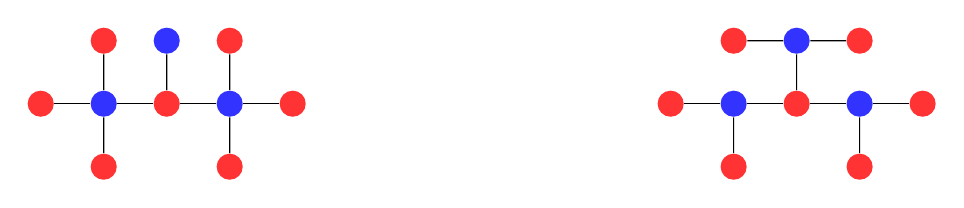
\begin{tikzpicture}
                [scale=.8,auto=left,every node/.style={circle}]
                \node [red] (n1) at (0,0) {};
                \node [blue](n2) at (1,0) {};
                \node [red] (n3) at (1,1) {};
                \node [red] (n4) at (1,-1){};
                \node [red] (n5) at (2,0) {};
                \node [blue](n6) at (2,1) {};
                \node [blue](n7) at (3,0) {};
                \node [red] (n8) at (3,1) {};
                \node [red] (n9) at (3,-1){};
                \node [red] (n0) at (4,0) {};
                
                \node [red] (m1) at (10,0){};
                \node [blue](m2) at (11,0){};
                \node [red] (m3) at (11,-1){};
                \node [red] (m4) at (12,0){};
                \node [blue](m5) at (12,1){};
                \node [red] (m6) at (11,1){};
                \node [red] (m7) at (13,1){};
                \node [blue](m8) at (13,0){};
                \node [red] (m9) at (14,0){};
                \node [red] (m0) at (13,-1){};
                
                \foreach \from/\to in {n1/n2,n2/n3,n2/n4,n2/n5,n5/n6,n5/n7,n7/n8,n7/n9,n7/n0}
                \draw (\from) -- (\to);
                
                \foreach \from/\to in {m1/m2,m2/m3,m2/m4,m4/m5,m5/m6,m5/m7,m4/m8,m8/m9,m8/m0}
                \draw (\from) -- (\to);
            \end{tikzpicture}
            \end{center}
            \hspace{12pt}\\
            
            \item \textit{Adapt an algorithm described in class so that it will determine whether a given undirected graph is bipartite. Give and justify its running time.}\\
            
            We shall adapt the Breadth-First Search algorithm. The principle is to check when dequeueing a vertex that all of its neighbors have either not be enqueued or are already the appropriate color.\\
            
            Without loss of generality, assume the graph $G$ has only one component. This assumption is justified since a graph with multiple components is bipartite if and only if each of its components is bipartite, due to the fact there are no edges between components.\\
             
            \newpage
            \begin{small}
            \begin{verbatim}
isBipartite(G):
    for i from 1 to n:
        v[i].color = WHITE      // mark each vertex white
        v[i].set = NULL
    
    Q = newFifo           // initialize FIFO queue
    
    v[1] = GREY       // pick a vertex and mark it
    v[1] = L          // put it in the set L
    Q.enqueue(1)      // enqueue it
    
    while Q not empty:
        x = Q.dequeue
        if v[x].set = L:
            opposite = R  // find the opposite set of x
        else 
            opposite = L
        
        for each neighbor y of x:
            if v[y].color == WHITE     // has not been touched
                v[y].color = GREY      // sets color to grey
                v[y].set = opposite    // puts in opposite set
                Q.enqueue(y)
                
            if v[y].set != opposite
                return FALSE        // two vertices of the same
                                    // set are next to each other
                                    
        v[x].color = BLACK
        
    return TRUE
                
        
            \end{verbatim}
            \end{small}
            
            The runtime of {\tt isBipartite} is $O(|V| + |E|)$, since its behavior is very similar to the {\tt searchTree} algorithm presented in class. The differences are determining sets $L$ and $R$, which is a constant time operation.
            
    \end{enumerate}
    
    \newpage
    \item \textit{(15 pts) Prof. Dumbledore needs your help to compute the in- and out-degrees of all vertices in a directed multigraph $G$. However, he is not sure how to represent the graph so that the calculation is most efficient. For each of the three possible representations, express your answers in asymptotic notation (the only notation Dumbledore understands), in terms of $V$ and $E$, and justify your claim.}
    \begin{enumerate}
         \item \textit{An edge list representation. Assume vertices have arbitrary labels.}
         
         $\Theta(|E|)$. This is because in order to compute the degrees of all the vertices, we must iterate through the entire edge list, of length $|E|$.\\
         
         \item \textit{An adjacency list representation. Assume the vector’s length is known.}
         
         $\Theta(|E|)$. This is for a similar reason. The number of edges has not changed, but the method still requires iterating over all of the edges. The order in which we do so is different.\\
         
         \item \textit{An adjacency matrix representation. Assume the size of the matrix is known.}
         
         $\Theta(|V|^2)$. To compute in-degrees, we sum each column, and to compute out-degrees, we sum each row. There are $|V|$ rows, each containing $|V|$ elements, so the total computations is $2|V|^2 = \Theta(|V|^2)$
         
    \end{enumerate}

\end{enumerate}

\newpage
\appendix
\section{Code}
\label{sec:code}
\subsection{Problem 1, part A}
\begin{Verbatim}[fontsize=\small]
import math
import io
from random import choice

'''
alignStrings(string x, string y)
Returns a cost matrix of alignment costs for turning x into y.
'''
def alignStrings(x, y):
    S = [[j+i for i in range(len(x)+1)] for j in range(len(y)+1)] # O(mn)

    print(len(x), len(y))

    for i in range(1, len(x)): # O(m)
        for j in range(1, len(y)): # O(n)
            cost = [0 for i in range(4)] #4 possible operations
            if(i > 2 and j > 2): #See if we could do a swap
                cost[0] = S[j-2][i-2] + 30 #Cost of a swap
            else:
                cost[0] = math.inf #This is only for the min function below, so
                                   #when a swap is impossible it won't pick it
            #print(j, i)
            if(x[i] == y[j]):
                cost[1] = S[j-1][i-1] #Nop, no additional cost
            else:
                cost[1] = S[j-1][i-1] + 10 #Cost of a sub

            cost[2] = S[j-1][i] + 1 #Cost of one indel
            cost[3] = S[j][i-1] + 1 #Cost of the other indel
            S[j][i] = min(cost)
    return(S)

'''
extractAlignment(matrix S)
Returns a vector of optimized operations to turn x into y.
'''
def extractAlignment(S, x, y):
    a = []
    [i,j] = [len(y) - 1, len(x) - 1]
    '''
    options: look up, left, diagonally up, and diag-up 2
    up -> i-1, j; cost 1
    left -> i, j-1; cost 1
    sub -> i-1, j-1; cost 10 or 0
    swap -> i-2, j-2; cost 30
    '''
    while [i, j] != [0,0]:
        options = []
        if i > 0:
            if S[i-1][j] == S[i][j] - 1: # up move possible
                options.append((('down', i, j, x[j], y[i]), (i-1, j)))

        if j > 0:
            if S[i][j-1] == S[i][j] - 1: # left move possible
                options.append((('right', i, j, x[j], y[i]), (i, j-1)))

        if i > 0 and j > 0: # could be a sub
            if S[i-1][j-1] == S[i][j] and x[j] == y[i]: #Make sure a nop is
                                                            # valid
                options.append((('nop', i, j, x[j], y[i]), (i-1, j-1)))

            if S[i-1][j-1] == S[i][j] - 10:
                options.append((('sub', i, j, x[j], y[i]), (i-1, j-1)))

        if i > 1 and j > 1:
            if S[i-2][j-2] == S[i][j] - 30: # and x[j-1] == y[i] and x[j] == y[i-1]:
                print('swep')
                options.append((('swap', i, j, x[j], y[i]), (i-2, j-2)))
        
        pick = choice(options)
        i,j = pick[1]
        a.append(pick[0])
    return a



'''
commonSubstrings(x,L,a)
a(x) -> y
Returns all substrings of x (length >= L) that align to a substring in y
'''
def commonSubstrings(x, L, a):
    #what should be returned?
    instring = 0 # Are we in a nop string of sufficent length?
    curstr = [] # The current array of nop letters
    same_strs = [] # A list of nop strings
    for op in reversed(a): # Since extractAlignment works from the end, flip
        if op[0] == 'nop':
            if instring == 1:
                same_strs[-1] += x[op[2]] # no newline
            elif len(curstr) >= L:
                instring = 1
                curstr.append(x[op[2]])
                same_strs.append(''.join(curstr)) # add that string to the 
                                                  #  current string (O(L))
                curstr = []
            else:
                curstr.append(x[op[2]])

        elif instring == 1:
            instring = 0
            curstr = []
        else:
            curstr = []
    return same_strs
\end{Verbatim}

\subsection{Problem 1, part F}
\begin{Verbatim}[fontsize=\small]
from random import choice
import math
import io

freqs = [[eval(j) for j in i.split(";")]
for i in open('csci3104_S2017_PS6_data_muchAdo_freqs.txt','r').read().split('\n')]
seed = ''.join([f[0]*f[1] for f in freqs])

def genString(n):
    return ''.join([choice(seed) for i in range(n)])

'''
alignStrings(string x, string y)
Returns a cost matrix of alignment costs for turning x into y.
'''
def alignStrings(x, y):
    S = [[j+i for i in range(len(x)+1)] for j in range(len(y)+1)] # O(mn)

    print(len(x), len(y))

    for i in range(1, len(x)): # O(m)
        for j in range(1, len(y)): # O(n)
            cost = [0 for i in range(4)] #4 possible operations
            if(i > 2 and j > 2): #See if we could do a swap
                cost[0] = S[j-2][i-2] + 30 #Cost of a swap
            else:
                cost[0] = math.inf #This is only for the min function below, so
                                   #when a swap is impossible it won't pick it
            #print(j, i)
            if(x[i] == y[j]):
                cost[1] = S[j-1][i-1] #Nop, no additional cost
            else:
                cost[1] = S[j-1][i-1] + 10 #Cost of a sub

            cost[2] = S[j-1][i] + 1 #Cost of one indel
            cost[3] = S[j][i-1] + 1 #Cost of the other indel
            S[j][i] = min(cost)
    return(S)

'''
extractAlignment(matrix S)
Returns a vector of optimized operations to turn x into y.
'''
def extractAlignment(S, x, y):
    a = []
    [i,j] = [len(y) - 1, len(x) - 1]
    '''
    options: look up, left, diagonally up, and diag-up 2
    up -> i-1, j; cost 1
    left -> i, j-1; cost 1
    sub -> i-1, j-1; cost 10 or 0
    swap -> i-2, j-2; cost 30
    '''
    while [i, j] != [0,0]:
        options = []
        if i > 0:
            if S[i-1][j] == S[i][j] - 1: # up move possible
                options.append((('down', i, j, x[j], y[i]), (i-1, j)))

        if j > 0:
            if S[i][j-1] == S[i][j] - 1: # left move possible
                options.append((('right', i, j, x[j], y[i]), (i, j-1)))

        if i > 0 and j > 0: # could be a sub
            if S[i-1][j-1] == S[i][j] and x[j] == y[i]: #Make sure a nop is
                                                            # valid
                options.append((('nop', i, j, x[j], y[i]), (i-1, j-1)))

            if S[i-1][j-1] == S[i][j] - 10:
                options.append((('sub', i, j, x[j], y[i]), (i-1, j-1)))

        if i > 1 and j > 1:
            if S[i-2][j-2] == S[i][j] - 30: # and x[j-1] == y[i] and x[j] == y[i-1]:
                print('swep')
                options.append((('swap', i, j, x[j], y[i]), (i-2, j-2)))

        pick = choice(options)
        i,j = pick[1]
        a.append(pick[0])
    return a



'''
commonSubstrings(x,L,a)
a(x) -> y
Returns all substrings of x (length >= L) that align to a substring in y
'''
def commonSubstrings(x, L, a):
    #what should be returned?
    instring = 0 # Are we in a nop string of sufficent length?
    curstr = [] # The current array of nop letters
    same_strs = [] # A list of nop strings
    for op in reversed(a): # Since extractAlignment works from the end, flip
        if op[0] == 'nop':
            if instring == 1:
                same_strs[-1] += x[op[2]] # no newline
            elif len(curstr) >= L:
                instring = 1
                curstr.append(x[op[2]])
                same_strs.append(''.join(curstr)) # add that string to the 
                                                  #  current string (O(L))
                curstr = []
            else:
                curstr.append(x[op[2]])

        elif instring == 1:
            instring = 0
            curstr = []
        else:
            curstr = []
    return same_strs

def checkForAlign(y, n):
    x = genString(n)
    print(x)
    common = commonSubstrings(x, 7, extractAlignment(alignStrings(x, y), x, y))
    return len(common) > 0

fx = io.open("./csci3104_S2017_PS6_data_muchAdo_txt.txt", 'r', encoding='utf8')
x = fx.read().encode('ascii', 'ignore').decode('ascii') # Strip all unicode

n = 300
good = False
while not good:
     n += 1
     good = checkForAlign(x, n)

print("minimum align is", n)

'''
Testing inputs
'''
fx = io.open("./csci3104_S2017_PS6_data_string_x.txt", 'r', encoding='utf8')
x = fx.read().encode('ascii', 'ignore').decode('ascii') # Strip all unicode

fy = io.open("./csci3104_S2017_PS6_data_string_y.txt", 'r', encoding='utf8')
y = fy.read().encode('ascii', 'ignore').decode('ascii') # Strip all unicode

#print(len(x), len(y))
#print(alignStrings(x, y)[len(y)][len(x)])
#print(extractAlignment(alignStrings(x, y), x, y))
common = commonSubstrings(x, 10, extractAlignment(alignStrings(x, y), x, y))
print(common)
print(len(common))
\end{Verbatim}


\section{List of Common Substrings}
\label{sec:substr}

A list of common substrings for Problem 1.

\begin{small}
\begin{verbatim}
' manufacturing '
' gulf coast '
'the companys '
' a keynote speech today '
', said woods. '
'mobil is strategically investing in new refining and 
    chemical-manufacturing projects in the u'
' gulf coast region to expand its manufacturing and 
    export capacity. the companys growing the gulf '
' consists of 11 major chemical, refining, lubricant 
    and liquefied natural gas projects at proposed new
    and existing facilities along the texas and 
    louisiana coasts. investments began in 2013 and 
    are expected to continue through at least 2022.  '
' to create '

\end{verbatim}
\end{small}

\end{document}

